% Section content template for individual Educative lessons
% This file contains the actual content for a specific section
% Generated from Educative API section content

% Section: In-Depth Investigation of CDN: Part 2
% Section ID: 5382114350727168
% Section Slug: in-depth-investigation-of-cdn-part-2
% Generated: 2025-12-07T17:14:25.099855

In this lesson, we learn how content consistency can be achieved using different consistency mechanisms. We also learn about where we should deploy the proxy servers and the difference between CDN as a service and specialized CDN.

\subsection{Content consistency in CDN}\label{XLAGLFpMJNmsVi2neKemE}
\\
Data in the proxy servers should be consistent with data in the origin servers. There 's always a risk of users accessing stale data if the proxy servers don't remain consistent with the origin servers. Different consistency mechanisms can be used to ensure consistency of data, depending on the push or pull model.

\subsubsection{Periodic polling}\label{tRLFLynzrpF_Ms8LZ4vt7}
\\
Using the pull model, proxy servers request the origin server periodically for updated data and change the content in the cache accordingly. When content changes infrequently, the polling approach consumes unnecessary bandwidth. Periodic polling uses \textbf{time-to-refresh (TTR)} to adjust the time period for requesting updated data from the origin servers.

\subsubsection{Time-to-live (TTL)}\label{IzZEDyxXQkHl2mv4d9inT}
\\
Because of the TTR, the proxy servers may uselessly request the origin servers for updated data. A better approach that could be employed to reduce the frequency of refresh messages is the \textbf{time-to-live (TTL)} approach. In this approach, each object has a TTL attribute assigned to it by the origin server. The TTL defines the expiration time of the content. The proxy servers serve the same data version to the users until that content expires. Upon expiration, the proxy server checks for an update with the origin server. If the data is changed, it gets the updated data from the origin server and then responds to the user's requests with the updated data. Otherwise, it keeps the same data with an updated expiration time from the origin servers.

\subsubsection{Leases}\label{Uzk4dLpUq5Jes3gFHnTzq}
\\
The origin server grants a lease to the data sent to a proxy server using this technique. The \textbf{lease} denotes the time interval for which the origin server agrees to notify the proxy server if there's any change in the data. The proxy server must send a message requesting a lease renewal after the expiration of the lease. The lease method helps to reduce the number of messages exchanged between the proxy and origin server. Additionally, the lease duration can be optimized dynamically according to the observed load on the proxy servers. This technique is referred to as an \textbf{adaptive lease}.
\\
In the following section, we discuss where to place the CDN proxy server to transmit data effectively.

\subsection{Deployment}\label{vf7jZLq1carBBBFYJr5fQ}
\\
We have to be clear with the answers to the following questions before we install the CDN facility:

\begin{itemize}
\item
\protect\phantomsection\label{woosKwbJoaysxSt8GPbzw}
What are the best locations to install proxy servers to maximally utilize CDN technology?
\item
\protect\phantomsection\label{k9sQwqUUrjnqJsO9fCXtx}
How many CDN proxy servers should we install?
\end{itemize}

\subsubsection{Placement of CDN proxy servers}\label{f70Q90KpxmLEzs43T9v5R}
\\
The CDN proxy servers must be placed at network locations with good connectivity. See the options below:

\begin{itemize}
\item
\protect\phantomsection\label{cIAvondxqBaUvg-8qe8DE}
\textbf{On-premises} represents a smaller data center that could be placed near major (IXPs)(An internet exchange point (IXP) is a physical infrastructure where multiple networks connect and exchange internet traffic directly to improve speed and reduce costs.).
\item
\protect\phantomsection\label{8GpkwrTxjO3BcK8i3hxX0}
\textbf{Off-premises} represents placing CDN proxy servers in ISPs(An internet service provider (ISP) is a company that provides individuals and organizations access to the internet and related services.)' networks.
\end{itemize}
\\
Today, it might be feasible to keep a large portion of a movie's data in a CDN infrastructure that's housed inside an ISP. Still , for services like YouTube, data is so large and ever-expanding that it's challenging to decide what we should put near a user. Google uses split TCP to reduce user-perceived delays by keeping persistent connections with huge TCP windows from the IXP-level infrastructure to their primary data centers. The client's TCP requests terminate at the IXP-level infrastructure and are then forwarded on already established, low latency TCP connections.
\\
Doing this substantially reduces client-perceived latency, which is due to the avoidance of the initial three-way handshake of TCP connection and slow-start stages to a host far away (had the client wanted to go to the primary data centers of Google). A round-trip delay to IXP is often very low. Therefore, three-way handshakes and slow starts at that level are negligible. \textbf{Predictive push} is a significant research field to decide what to push near the customers.
\\
We can use measurements to facilitate the decision of proxy server placement. One such tool is \textbf{ProxyTeller}(A proxy placement tool for content delivery under performance constraints. Source: Trianfillou, P. and Aekaterinidis, I., 2003, December. Proceedings of the Fourth International Conference on Web Information Systems Engineering, 2003. WISE 2003. (pp. 62-71). IEEE.) to decide where to place the proxy server and how many proxy servers are required to achieve high performance. ProxyTeller uses hit ratio, network bandwidth, and client-response time (latency) as performance parameters to decide the placement of proxy servers. Other greedy, random, and hotspot algorithms are also used for proxy server placements.
\begin{quote}
\textbf{Note}: Akamai and Netflix popularized the idea of keeping their CDN proxy servers inside the client's ISPs. For many clients of Akamai, content is just one network hop away. On the other hand, Google also has its private CDN infrastructure but relies more on its servers near IXPs. One reason for this could be the sheer amount of data and the change patterns.
\end{quote}

\begin{quote}
\textbf{Quiz:}
\textbf{Question 1:} What benefits could an ISP get by placing the CDN proxy servers inside their network?
\textbf{Answer:} A CDN node cuts down the amount of external bandwidth that ISPs need and pay for. The SLA defined by ISPs with the proxy server providers may benefit the ISPs economically. A CDN node improves responsiveness for the ISP's customers, which makes the ISP's customers happier. This gives them a competitive advantage over ISPs that don't have a CDN node.

Bringing content closer to the users reduces data on the Internet core.
\end{quote}

\subsection{CDN as a service}\label{B1OUCDbXaWcUIaZOZb6ev}
\\
Most companies don't build their own CDN. Instead , they use the services of a CDN provider, such as Akamai, Cloudflare, Fastly, and so on, to deliver their content. Similarly
, players like AWS make it possible for anyone to use a global CDN facility.
\\
The companies sign a contract with the CDN service provider and deliver their content to the CDN, thereby allowing the CDN to distribute the content to the end users. A public CDN raises the following concerns for content providers:

\begin{itemize}
\item
\protect\phantomsection\label{X4FgavYB-3W0Ua4_3Wjv_}
The content provider can't do anything if the public CDN is down.
\item
\protect\phantomsection\label{3ofu3ZGwNXl3eXr_Ed6oq}
If a public CDN doesn't have any proxy servers located in the region or country where some website traffic comes from, then those specific customers are out of luck. In such cases, the content providers have to buy CDN services from other CDN providers or deploy and use their own private CDN.
\item
\protect\phantomsection\label{Hqw76hPacc8FQ0cA0j8VA}
It's possible that some domains or IP addresses of CDN providers are blocked or restricted in some countries because they might be delivering content that's banned in those countries.
\end{itemize}
\begin{quote}
\textbf{Note}: Some companies make their own CDN instead of using the services of CDN providers. For example, Netflix has its own purpose-built CDN called \textbf{Open Connect}.
\end{quote}
\subsection{Specialized CDN}\label{GWfvHJVNxbI3MX021_IWM}
\\
We've discussed that many companies use CDN as a service, but there are cases where companies build their own CDN. A number of reasons factor into this decision. One is the cost of a commercial CDN service. A specialized CDN consists of points of presence \textbf{(PoPs)} that only serve content for their own company. These PoPs can be caching servers, reverse proxies, or application delivery controllers. Although a specialized CDN has high costs at its first setup, the costs eventually decrease with time. In essence, it's a buy versus build decision.
\\
The specialized CDN's PoPs consist of many proxy servers to serve petabytes of content. A private CDN can be used in coexistence with a public CDN. In case the capacity of a private CDN isn't enough or there's a failure that leads to capacity reduction, the public CDN is used as a backup. Netflix's \textbf{Open Connect Appliance (OCA)} is an example of a CDN that's specialized in video delivery.
\\
Netflix's OCA servers don't store user data. Instead, they fulfill the following tasks:

\begin{itemize}
\item
\protect\phantomsection\label{PWMUZ2MPZroB_Rr74G1Zt}
They report their status---health, learned routes, and details of cached content---to the Open Connect control plane that resides in AWS (Amazon Web Services).
\item
\protect\phantomsection\label{y9kmeVweJzhPINQx5MBoi}
They serve the cached content that's requested by the user.
\end{itemize}

\begin{figure}[htbp]
 \centering
 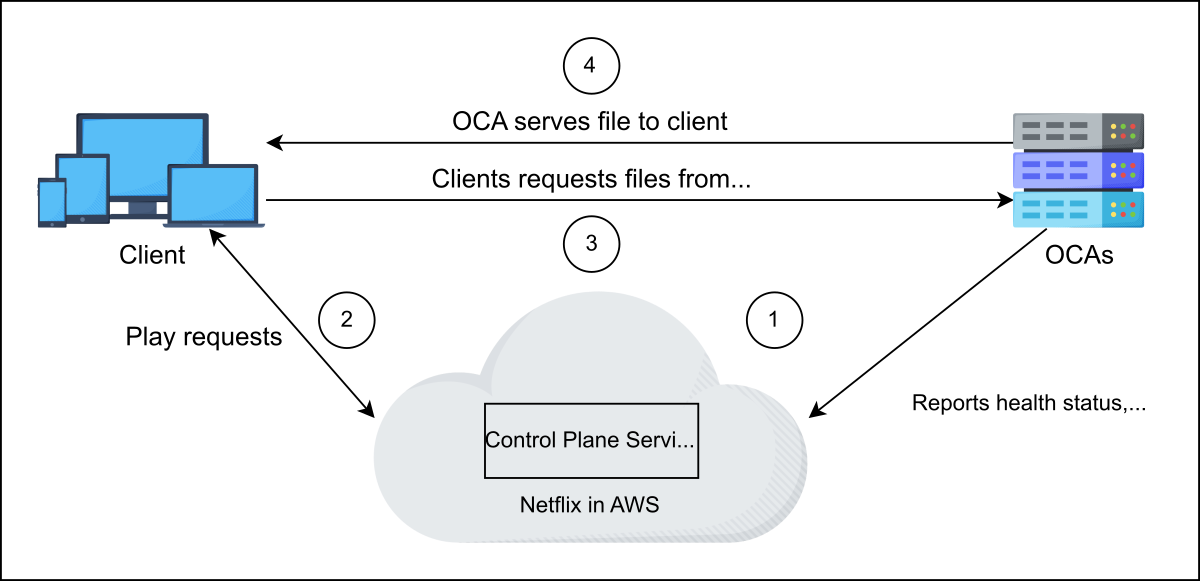
\includegraphics[width=0.5\textwidth]{Images/chapter_11/section_5382114350727168/6641190122684416.png}
 \caption{Netflix's Open Connect Appliances}
\end{figure}

All the deployed OCAs situated in IXP or embedded in the ISP network are monitored by the Open Connect operation team.

\subsubsection{Why Netflix built its CDN}\label{mJ42bBApi7Dj7UVRFv5gr}
\\
As Netflix became more popular, it decided to build and manage its own CDN for the following reasons:

\begin{itemize}
\item
\protect\phantomsection\label{YUKLcEb_xOrfAiZUlVwcM}
The CDN service providers were scuffling to expand their infrastructure due to the rapid growth in customer demand for video streaming on Netflix.
\item
\protect\phantomsection\label{y5N_jeRlMgWfKQkSqXczj}
With the increasing volume of streaming videos, the expense of using CDN services increased.
\item
\protect\phantomsection\label{ChQiFVvDuAJ4k5Zav4pYU}
Video streaming is the main business and a primary revenue source for Netflix. So , protecting the data of all the videos on the platform is critical. Netflix
's OCA manages potential data leakage risks in a better way.
\item
\protect\phantomsection\label{9uQ-5xfI9jCvdtu2pqiYi}
To provide optimal streaming media delivery to customers, Netflix needed to maximize its control over the user's video player, the network between the user, and the Netflix servers.
\item
\protect\phantomsection\label{w_EgRgRlvgtWAqhAZhbV7}
Netflix's OCA can use custom HTTP modules and TCP connection algorithms to detect network problems quickly and troubleshoot any issues in their CDN network.
\item
\protect\phantomsection\label{inmeR_Ca-Z1wbiTo_3XQt}
Netflix wanted to keep popular content for a long time. This wasn't entirely possible while operating with a public CDN due to the high costs that would be incurred to keep and maintain it.
\end{itemize}
\begin{quote}
\textbf{Note}: Netflix is able to achieve a hit ratio close to 95\% using OCA.
\end{quote}
\\
We'll evaluate our proposed design in the next lesson.

% End of section content